\documentclass[conference]{IEEEtran}
\usepackage{amsmath,amssymb}
\usepackage{graphicx}
\usepackage{booktabs}
\usepackage{array}
\usepackage{url}
\usepackage{cite}
\usepackage{algorithm}
\usepackage{algpseudocode}
\usepackage{tikz}
\usetikzlibrary{positioning}

% include a table generated by make_tables.py, or a visible warning if it is missing
\newcommand{\maybeinput}[1]{\IfFileExists{#1}{\input{#1}}{\par\textbf{[missing #1: run make\_tables.py]}\par}}
% include a figure, or a visible placeholder box if the file is missing
\newcommand{\figorbox}[2]{\IfFileExists{#1}{\includegraphics[width=#2]{#1}}{\fbox{\parbox{#2}{\centering\small [missing figure: \detokenize{#1}]}}}}

\begin{document}

\title{Criterion-Level Clinical Trial Eligibility Screening with a LoRA-Fine-Tuned Qwen2.5 Decoder: Evidence Citation, KV-Cached and Speculative Decoding, and Tiled Attention}

\author{\IEEEauthorblockN{Hamna Asif}
\IEEEauthorblockA{Roll No.\ 23I-0658, Section G, Generative AI (Assignment 2)\\
FAST NUCES, Islamabad, Pakistan\\
hamnaasif7377@gmail.com}}

\maketitle

\begin{abstract}
We build and evaluate a complete, locally executable system that matches a patient description to individual inclusion and exclusion criteria of clinical trials. A Qwen2.5-1.5B-Instruct decoder is fine-tuned with LoRA on the patient-grouped training split (37 patients) of the TrialGPT Criterion Annotations and outputs a structured JSON answer: one of the dataset's expert label categories and the IDs of the supporting patient sentences. On the held-out test split (8 patients, 206 criterion records) the fine-tuned model reaches 0.733 accuracy and 0.540 macro-F1, against 0.170/0.141 for the same base model prompted zero-shot with the label list; evidence macro-F1 rises from 0.587 to 0.835. The dominant failure is that missing information is read as ``not excluded''. We also implement, from scratch and without \texttt{generate()}, a KV-cached greedy decoder (token-identical to the uncached reference in float32; up to 5.6$\times$ faster at 1024 input tokens), a tiled online-softmax attention (error $\approx10^{-16}$ in float64, 384 MB $\rightarrow$ 6 MB peak memory at length 2048), and a greedy speculative decoder (token-identical, acceptance 0.96, but 0.68--0.72$\times$ the speed of plain cached decoding on a T4). Everything is exposed through a browser application with evidence inspection, report export and a live benchmark view. The system is an educational screening prototype, not a clinical decision tool.
\end{abstract}

\begin{IEEEkeywords}
clinical trial matching, eligibility criteria, large language models, LoRA, KV cache, online softmax, speculative decoding
\end{IEEEkeywords}

\section{Introduction}
Deciding whether a patient satisfies each inclusion and exclusion criterion of a clinical trial is slow manual work. Large language models can read the free-text criteria and the patient note, but a useful screening tool must (i) preserve the expert label scheme, including \emph{not enough information} and \emph{not applicable}, (ii) point to the exact patient sentences behind each decision, and (iii) run on modest, freely accessible hardware.

This paper documents a single-author implementation of such a tool and of the Transformer inference mechanisms it relies on. The contributions are:
\begin{itemize}
\item A LoRA fine-tuning pipeline on the prescribed TrialGPT Criterion Annotations \cite{jin2024trialgpt}, with a fixed patient-grouped 37/8/8 split, leakage checks, and a before/after comparison on identical examples.
\item A criterion-level pipeline that returns label, cited sentence IDs, extracted evidence text and a templated explanation, evaluated with accuracy, macro-F1, per-class metrics, confusion matrices and evidence precision/recall/F1.
\item A hand-written KV-cached decoder, a tiled online-softmax attention and a greedy speculative decoder, each verified against a reference and benchmarked honestly, including where they are \emph{slower}.
\item A browser application that runs all of the above and exports a screening report.
\end{itemize}
The dataset provides criterion-level labels only; any patient-level outcome shown by our application is an explicit rule-based aggregation (Section~\ref{sec:app}), not a labeled ground truth.

\section{Related Work}
\textbf{Trial matching.} TrialGPT \cite{jin2024trialgpt} prompts GPT-4 to produce criterion-level eligibility, explanations and evidence sentences, and ranks trials by aggregating these; its annotation set is our mandatory benchmark. The patient cohorts descend from the SIGIR 2016 trial-matching collection \cite{koopman2016test}. TrialGPT relies on a proprietary API; we instead adapt a small open-weight model and compare it to the same model without adaptation. We never feed the GPT-4 predictions or explanations contained in the dataset to our model.

\textbf{Parameter-efficient adaptation.} LoRA \cite{hu2022lora} freezes the pretrained weights and trains low-rank updates, which fits a 1.5B model on a free 15~GB T4. QLoRA \cite{dettmers2023qlora} adds 4-bit quantization; we did not need it because the fp16 model fits, and it would complicate the later merged-weights decoding experiments.

\textbf{Efficient inference.} Decoder-only Transformers \cite{vaswani2017attention} generate one token at a time, and autoregressive decoding reuses cached keys and values \cite{pope2023efficiently}; Qwen2.5 uses grouped-query attention \cite{ainslie2023gqa} and rotary embeddings \cite{su2024roformer}, which shape the cache layout and position handling. The online normalizer \cite{milakov2018online} underlies FlashAttention \cite{dao2022flashattention}, which tiles attention to avoid materializing the $L\times L$ score matrix. Speculative decoding \cite{leviathan2023fast,chen2023accelerating} lets a small draft model propose tokens that a large target model verifies in one pass. Its speedup depends on the draft/target cost ratio and the acceptance rate, which is why we measure both.

\textbf{Model families.} Qwen2.5 \cite{qwen2024qwen25}, Llama 3 \cite{dubey2024llama3} and Gemma 2 \cite{gemma2024gemma2} are the open-weight decoder families we compared (Section~\ref{sec:model}).

\section{Materials and Methods}
\begin{figure}[t]
\centering
\resizebox{\columnwidth}{!}{%
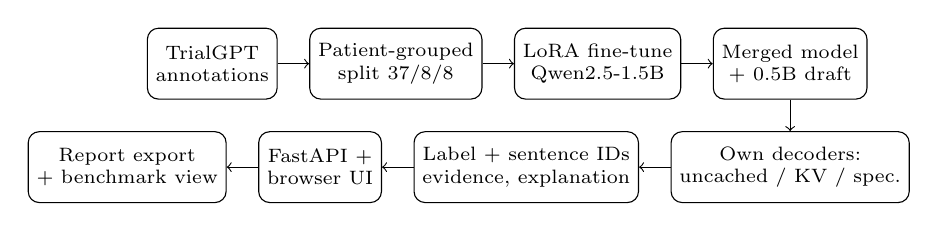
\begin{tikzpicture}[node distance=4mm, box/.style={draw, rounded corners, align=center, font=\scriptsize, minimum height=9mm, inner sep=3pt}]
\node[box] (a) {TrialGPT\\annotations};
\node[box, right=of a] (b) {Patient-grouped\\split 37/8/8};
\node[box, right=of b] (c) {LoRA fine-tune\\Qwen2.5-1.5B};
\node[box, right=of c] (d) {Merged model\\+ 0.5B draft};
\node[box, below=of d] (e) {Own decoders:\\uncached / KV / spec.};
\node[box, left=of e] (f) {Label + sentence IDs\\evidence, explanation};
\node[box, left=of f] (g) {FastAPI +\\browser UI};
\node[box, left=of g] (h) {Report export\\+ benchmark view};
\draw[->] (a)--(b); \draw[->] (b)--(c); \draw[->] (c)--(d); \draw[->] (d)--(e);
\draw[->] (e)--(f); \draw[->] (f)--(g); \draw[->] (g)--(h);
\end{tikzpicture}}
\caption{System overview from data to application.}
\label{fig:arch}
\end{figure}

\subsection{Dataset, split and leakage control}
The TrialGPT Criterion Annotations hold 1015 rows from 53 patients. Each row has a patient note whose sentences are numbered, a trial and one criterion with its type, the expert eligibility label and the expert evidence sentence IDs. The columns \texttt{gpt4\_explanation}, \texttt{gpt4\_sentences}, \texttt{gpt4\_eligibility} and \texttt{explanation\_correctness} are dropped during preprocessing and never reach the model or the metrics. We ignore the dataset's own \texttt{training} flag.

Unique patient IDs are sorted, shuffled with \texttt{numpy.random.default\_rng(42)}, and the first 37, next 8 and last 8 form train, validation and test. All annotations of a patient stay in one split. The script asserts that the three patient sets are disjoint, that no record is lost or duplicated, and that annotation IDs are unique; it saves the manifest (patient IDs and counts) as \texttt{manifests/split\_manifest.json}. The test split was run once, after all design decisions, and no threshold or prompt was tuned on it.

\begin{table}[t]
\centering\footnotesize
\caption{Split statistics. ``Empty gold'' counts records whose expert evidence list is empty.}
\label{tab:split}
\begin{tabular}{lrrrr}\toprule
Split & Patients & Records & Empty gold & Mean sentences\\\midrule
Train & 37 & 603 & 349 & 6.1\\
Validation & 8 & 206 & 116 & 7.1\\
Test & 8 & 206 & 145 & 5.7\\\bottomrule
\end{tabular}
\end{table}

Table~\ref{tab:split} shows that most records have no gold evidence, so the evidence metric needs an explicit empty-set rule (Section~\ref{sec:metrics}). The labels are strongly imbalanced: in training, exclusion criteria are 292 \emph{not excluded}, 65 \emph{not enough information}, 23 \emph{not applicable} and only 8 \emph{excluded}; inclusion criteria are 109 \emph{not enough information}, 88 \emph{included}, 13 \emph{not included} and 5 \emph{not applicable}. The test split has no \emph{excluded} record at all (exclusion: 91 \emph{not excluded}, 28 NEI, 12 NA; inclusion: 27 included, 7 not included, 38 NEI, 3 NA).

\subsection{Candidate models and selection}\label{sec:model}
\begin{table}[t]
\centering\footnotesize
\caption{Open-weight decoder candidates (figures from the model cards; fp16 weight size $\approx$ 2 bytes $\times$ parameters).}
\label{tab:models}
\begin{tabular}{@{}p{1.75cm}p{0.9cm}p{1.2cm}p{0.9cm}p{2.0cm}@{}}\toprule
Model & Params & Licence & Context & Notes\\\midrule
Qwen2.5-1.5B-Instruct & 1.54B & Apache-2.0 & 32k & 28 layers, GQA (2 KV heads), vocab 151,936; $\approx$3.1 GB\\
Qwen2.5-0.5B-Instruct & 0.49B & Apache-2.0 & 32k & same tokenizer; $\approx$1.0 GB; used as draft\\
Llama-3.2-1B & 1.2B & Llama community (gated) & 128k & different tokenizer (128k vocab)\\
Gemma-2-2B & 2.6B & Gemma terms & 8k & 256k vocab; $\approx$5.2 GB\\\bottomrule
\end{tabular}
\end{table}
We chose \textbf{Qwen2.5-1.5B-Instruct} as the target and \textbf{Qwen2.5-0.5B-Instruct} as the speculative draft (Table~\ref{tab:models}). Reasons: (i) a permissive licence and no access gate, so the grader can reproduce everything; (ii) the 0.5B and 1.5B models share one tokenizer (verified in code by comparing the two vocabularies), which speculative decoding requires; (iii) the fp16 weights (2.9~GiB) leave ample room on a 15~GB T4 for LoRA training with gradient checkpointing, and the merged fp32 model ($\approx$6.2~GB) runs on a CPU laptop for the application; (iv) a 32k context is far above the longest prompt we see (562 tokens). We considered Gemma-2-2B (twice the memory, 8k context, different vocabulary, no smaller same-tokenizer draft in our setup) and the Llama-3.2 family (gated licence; it would require a larger target to pair with the 1B draft). We did not train these two, so we make no empirical claim about them. T4 GPUs lack bfloat16, so we train and decode in fp16 with fp32 LoRA weights, and use PyTorch's SDPA rather than FlashAttention-2.

\subsection{Input/output format, tokenization and truncation}
Each example is a chat prompt built with the model's chat template: a fixed system instruction, the numbered patient note, the criterion type and the criterion text. The target is a compact JSON object \texttt{\{"label": ..., "evidence\_sentence\_ids": [...]\}}. We deliberately do not train the model to write an explanation: the application builds it deterministically from the cited sentences, so it is always traceable to the record and never invented, and the output stays short (about 16 tokens), which helps the decoding experiments. Loss is computed only on the answer tokens (prompt tokens are masked with $-100$). The maximum sequence length was set to 1536 tokens. Token statistics (prompt plus answer): train mean 267, 95th percentile 433, maximum 562; validation mean 280, maximum 396; test mean 250, maximum 456. No record exceeds 1024 tokens, so \textbf{no example was truncated} in training, validation or test, and no evidence sentence could have been cut away.

\subsection{Fine-tuning}
We train LoRA adapters on all seven projection matrices (q, k, v, o, gate, up, down) with rank 16, $\alpha=32$ and dropout 0.05: 18,464,768 trainable parameters, 1.18\% of the model. Settings: AdamW via the Hugging Face Trainer, learning rate $2\times10^{-4}$ with cosine decay and 5\% warm-up, per-device batch 4 with 4 accumulation steps (effective batch 16), 3 epochs (114 optimizer steps), fp16 mixed precision with fp32 adapter weights, gradient checkpointing, seed 42, checkpoint and validation-loss evaluation every epoch with the best epoch restored. The script resumes from the last checkpoint on Google Drive, so training could continue across free Colab sessions and accounts. Training took 589~s on a T4. The draft model uses the same recipe: 8,798,208 trainable parameters, 282~s.

Alternatives considered and rejected: full fine-tuning (memory, and 603 examples would overfit); 4-bit QLoRA (unnecessary at this size); an ONNX export (our cache and speculative loops need direct PyTorch access to the model); generating free-text explanations (slower decoding and hallucination risk). Only one LoRA configuration was trained for lack of time, so no hyperparameter search is reported.

\subsection{KV-cached decoding}
Both decoders call the bare transformer (\texttt{model.model}) and the \texttt{lm\_head} directly; \texttt{generate()} is never used. The \emph{reference} re-runs the whole sequence for every new token. The \emph{cached} decoder prefills the prompt once while filling a \texttt{DynamicCache}, then feeds one token per step. Three details need care.
\begin{itemize}
\item \textbf{Positions.} Rotary embeddings need the absolute index of each token. For a chunk starting at position $p$ we pass \texttt{position\_ids} $=p,\dots,p+n-1$, where $p$ is the current cache length. Passing positions $0..n-1$ would silently corrupt every cached step.
\item \textbf{Masking.} The attention mask spans cache plus new tokens (batch of one, no padding, so all ones); causality inside a multi-token chunk (the prefill, or the speculative verify pass) is applied by the model.
\item \textbf{Cache growth.} Each layer appends the new keys and values. With 28 layers, 2 KV heads and head dimension 128, the cache costs $28\cdot2\cdot2\cdot128\cdot2=28{,}672$ bytes per token in fp16 (6.3~MB for 220 tokens), small thanks to grouped-query attention.
\end{itemize}
Cached and uncached paths can differ numerically because they multiply differently shaped matrices (one row versus the full sequence), so accumulation order and fp16 rounding differ. A greedy argmax flips only when the top-two logits are nearly tied.

\subsection{Tiled attention with online softmax}
The reference computes $S=QK^\top/\sqrt d$, applies the causal mask, subtracts the row maximum, exponentiates and normalizes. The tiled version processes query blocks and key blocks and never forms the full $S$. For each query row it keeps a running maximum $m$, normalizer $\ell$ and output accumulator $a$. For a new key block with scores $s_j$ and values $v_j$:
\begin{align}
m' &= \max\bigl(m,\max_j s_j\bigr), \quad \alpha=e^{m-m'},\nonumber\\
\ell &\leftarrow \alpha\ell+\textstyle\sum_j e^{s_j-m'}, \quad
a \leftarrow \alpha a+\textstyle\sum_j e^{s_j-m'}v_j,
\end{align}
and the output is $a/\ell$. Queries sit at absolute position $i+(L_k-L_q)$, so a short query block attending to a longer key/value set (the cached-decoding situation) is masked correctly; key blocks entirely above the diagonal are skipped, and fully masked rows are handled without producing NaNs. The code computes in float32 (or float64 for float64 inputs).

\subsection{Greedy speculative decoding}
\begin{algorithm}[t]
\caption{One round of greedy speculative decoding}\label{alg:spec}
\begin{algorithmic}[1]
\State \textbf{Invariant:} both caches hold the sequence without its last token $x$ (pending)
\State $d_1\ldots d_k \gets$ draft greedy tokens, feeding $x$ then each $d_i$
\State logits $\gets$ target forward over $[x,d_1,\ldots,d_k]$ (one pass)
\State $g_i \gets \arg\max$ logits$_i$; $m \gets$ longest prefix with $d_{i+1}=g_i$
\State append $d_1\ldots d_m$ and $g_m$ (correction if $m<k$, bonus if $m=k$)
\State crop the target cache to the accepted prefix
\State draft cache: crop on rejection, or feed the one unseen $d_k$ on full acceptance
\end{algorithmic}
\end{algorithm}
Algorithm~\ref{alg:spec} gives one round. Every round emits $m+1\ge1$ tokens and the output equals plain greedy decoding of the target. We wrote the cache trimming ourselves because the library's \texttt{crop} semantics changed between versions (a positive length was rejected by the Colab version); our wrapper removes the surplus tokens explicitly. The draft is Qwen2.5-0.5B fine-tuned on the same training split, and an untuned draft is used as a comparison.

\subsection{Application workflow}\label{sec:app}
The application is a FastAPI back end with a single-page browser UI (no code has to be run by the user). A user pastes a patient note (numbered, or plain text that is split into sentences automatically), selects or types criteria under ``Inclusion criteria:'' / ``Exclusion criteria:'' headers, picks the decoding path, and runs. For each criterion it shows the label, the cited sentences (highlighted in the note), a templated explanation, warnings and the raw model output. Invalid input (empty note, no header, too many criteria, over-long text, unknown mode) returns a readable message and keeps the user's text. Warnings flag invalid JSON, labels not valid for the criterion type, cited IDs outside the note, decisions without cited evidence (for \emph{not excluded} this may only mean the note never mentions the criterion), and prompts longer than any training example. The overall preliminary outcome is an explicit rule: any \emph{not included} inclusion or \emph{excluded} exclusion criterion gives ``Likely ineligible''; otherwise any invalid output gives ``Needs manual review''; otherwise any \emph{not enough information} gives ``Undetermined''; otherwise ``Preliminarily eligible''. Missing information is never treated as eligibility or ineligibility. A standalone HTML report (and JSON) with provenance (model, adapter, decoding mode, device, note hash, timing) is saved and downloadable. A visible notice states that this is an educational screening prototype and not a clinical enrollment decision. The benchmark tab runs one criterion through the uncached, KV-cached and speculative paths live and compares time, tokens/s and token equality; the experiments tab renders the recorded results and runs a live attention check. Start-up uses \texttt{python -m uvicorn app.main:app} or Docker Compose (Section~\ref{sec:repro}).

\section{Experimental Setup and Metrics}\label{sec:metrics}
\textbf{Hardware.} Training and the main benchmarks ran on a free Google Colab Tesla T4 (15~GB, fp16, PyTorch SDPA). The application ran on a Windows laptop without a GPU (8 CPU threads, fp32). Exact library versions are in the repository's lock file.

\textbf{Decoding for evaluation.} Greedy decoding, at most 64 new tokens, batch size 8, fp16, identical for the base and fine-tuned models. The base model is evaluated with two prompts: the \emph{naive} prompt used for fine-tuning, and a \emph{hint} prompt that additionally lists the allowed labels, because the naive prompt does not tell the base model the label vocabulary.

\textbf{Label metrics.} Accuracy, macro-F1, per-class precision/recall/F1 and confusion matrices, overall and separately for inclusion and exclusion. Macro-F1 averages over classes that occur in the gold labels or the predictions, so a class absent from both (\emph{excluded} in the test split) does not count as an automatic zero. Unparsable or out-of-vocabulary outputs are mapped to an INVALID class and count as errors.

\textbf{Evidence metrics.} Per record, precision, recall and F1 between predicted and gold sentence-ID sets. If both sets are empty the record scores 1 (correct abstention); if exactly one is empty it scores 0. We report macro averages over records, micro averages over all sentences, and macro-F1 restricted to records with non-empty gold evidence. Absent evidence is never taken as proof of eligibility or ineligibility.

\textbf{Timing.} Two warm-up runs, CUDA synchronization around every timed region, median of repeated runs, and \texttt{ignore\_eos} so that all paths produce exactly the requested number of tokens. Prefill time is the first step, decode time the rest. Peak memory is the CUDA allocator maximum.

\section{Results and Discussion}
\subsection{Training}
\begin{figure}[t]
\centering
\figorbox{figures/training_curves.png}{0.9\columnwidth}
\caption{Training and validation loss of the LoRA run.}
\label{fig:curves}
\end{figure}
Fig.~\ref{fig:curves} shows that the training loss falls from 1.0 to about 0.05 and that the model learns the JSON format within roughly ten steps (0.22 at step 10). Validation loss was 0.1386, 0.1117 and 0.1154 after epochs 1, 2 and 3: it is lowest at epoch 2 and rises slightly at epoch 3 while training loss keeps falling, the start of overfitting on 603 examples. The saved adapter is therefore the epoch-2 checkpoint. For the draft model the validation loss was 0.1595, 0.1337 and 0.1270, still improving at epoch 3.

\subsection{Before and after fine-tuning}
\maybeinput{tab_main_val.tex}
\maybeinput{tab_main_test.tex}
Tables~\ref{tab:val} and~\ref{tab:test} compare the same base model before and after fine-tuning on identical examples and decoding settings. With the naive prompt the base model scores exactly 0 accuracy even though its JSON is always valid, because it answers ``Eligible'' or ``Ineligible'', which are not dataset labels; this baseline is therefore uninformative, which is why we added the hint prompt. Even with the labels listed, the base model reaches only 0.170 accuracy on the test split, mostly by predicting \emph{excluded} or \emph{not applicable}. Fine-tuning raises test accuracy to 0.733 and macro-F1 to 0.540, and evidence macro-F1 from 0.587 to 0.835, with 100\% valid JSON in all runs. Test macro-F1 (0.540) is higher than validation (0.407); a main reason is that the test split contains no \emph{excluded} record, so that hard class drops out of the average. With eight test patients the difference is within noise, and we do not claim better generalization on test. We report no confidence intervals and a single run.

\begin{figure}[t]
\centering
\figorbox{figures/test_comparison.png}{\columnwidth}
\caption{Test accuracy, macro-F1 and evidence macro-F1 for the three configurations, overall, inclusion and exclusion.}
\label{fig:comparison}
\end{figure}
Fig.~\ref{fig:comparison} visualizes the same comparison.

\subsection{Per-class behaviour and confusion}
\maybeinput{tab_perclass.tex}
\maybeinput{tab_conf.tex}
\begin{figure}[t]
\centering
\figorbox{figures/test_confusion_finetuned.png}{0.85\columnwidth}
\caption{Overall test confusion matrix of the fine-tuned model.}
\label{fig:confusion}
\end{figure}
Table~\ref{tab:perclass}, Table~\ref{tab:conf} and Fig.~\ref{fig:confusion} show where the remaining errors are. \emph{Not excluded} is recognized almost perfectly (89 of 91) and \emph{included} with perfect precision (20 of 27 recalled). The 55 test errors are dominated by 28 \emph{not enough information} records predicted as \emph{not excluded}, 7 \emph{included} and 7 \emph{not included} records predicted as NEI, and 8 \emph{not applicable} records predicted as \emph{not excluded}. The rare classes are the weak point: \emph{not included} (7 test records) is never predicted correctly and \emph{not applicable} reaches only 4 of 15. Training had 13 \emph{not included}, 8 \emph{excluded} and 5 inclusion-NA examples, so the model has barely seen them. Inclusion and exclusion criteria behave differently: inclusion accuracy is 0.773 against 0.710 for exclusion, but exclusion has the strongest evidence retrieval (Table~\ref{tab:evidence}) and is dominated by the over-confident \emph{not excluded} prediction.

\subsection{Evidence localization}
\maybeinput{tab_evidence.tex}
Table~\ref{tab:evidence} reports evidence retrieval. Because 70\% of the test records have no gold evidence (Table~\ref{tab:split}), the macro scores reward correct abstention; the non-empty columns show the harder case of locating sentences when evidence exists. The fine-tuned model clearly beats both baselines. Typical failures are over-citation (extra neighbouring sentences) and spurious citations for criteria the note does not address (cases 5 and 8 below).

\subsection{Error analysis}
\begin{table*}[t]
\centering\footnotesize
\caption{Distinct test errors of the fine-tuned model (annotation IDs refer to the dataset).}
\label{tab:errors}
\begin{tabular}{@{}p{0.9cm}p{4.6cm}p{2.3cm}p{2.3cm}p{5.8cm}@{}}\toprule
ID & Criterion & Gold & Predicted & Observation\\\midrule
389--412 (24 cases) & e.g.\ ``Drug abuse'', ``Major surgery within 3 weeks'', ``Vaccination within 4 weeks'' & NEI, no evidence & not excluded, no evidence & Missing information read as eligibility; the dominant failure: 28 of the 55 test errors are NEI predicted as \emph{not excluded}, and these 24 cases plus 193, 315, 756 and 849 make up that group.\\
193 & ``Patients were moribund'' & NEI, evidence [0--4] & not excluded, none cited & The note lists shock-like findings (BP 80/60, tachycardia); the model cites nothing and decides ``not excluded''.\\
176 & ``No medical history of central vena catheterization'' & included, [0] & NEI, [0] & Right sentence, wrong label: a negated inclusion criterion confuses the model.\\
186, 187 & ``Heart rate of at least 90/min''; ``respiratory rate of at least 20/min\ldots'' & included, [2] & NEI, [2] & Right evidence (``tachycardic/tachypneic'') but the model cannot map a qualitative word to a numeric threshold.\\
162--164 & Surgical procedures (open AAA repair, endovascular repair, lower limb revascularisation) & not included, no evidence & NEI, cites [0,1,2] & Spurious evidence: three unrelated sentences about a femoral-artery complication are cited.\\
322 & ``Pregnant women or women of childbearing age\ldots'' (male patient) & not excluded, [0] & not applicable, none & Applicability by patient sex handled inconsistently with the annotators.\\
767, 771 & ``Females of childbearing potential'' (5-year-old boy) & not applicable, [0] & not excluded, none & NA confused with the negative exclusion label; evidence missed.\\
850 & Asthma exacerbation more than 2x/week & not excluded, [0,1,3,6] & NEI, [0,1,2,3,4] & Over-cited evidence and over-cautious label.\\
836 & Asthma after age 6 years & not included, [0,1] & NEI, [0,1,3,4] & Correct core evidence plus two irrelevant sentences; the rare label \emph{not included} is missed.\\
849 & Night-time cough/wheeze more than 1x/week & NEI, [0,3,6] & not excluded, [1,2,3,4] & Wrong label and mostly wrong sentences.\\\bottomrule
\end{tabular}
\end{table*}
Table~\ref{tab:errors} lists more than eight distinct errors. Three patterns stand out. (1) \emph{Missing information becomes ``not excluded''.} The model rarely says that a criterion is unaddressed; the application therefore flags every \emph{not excluded} decision that cites no sentence. (2) \emph{Numeric and negated criteria.} The model finds the right sentence but cannot compare numbers or handle negation reliably. The live application shows this: for a note stating HbA1c 8.2\% and BMI 31 it answered NEI for ``HbA1c between 7.5\% and 10\%'' and ``BMI above 25'' while citing the correct sentence. (3) \emph{Rare labels.} \emph{Not included}, \emph{excluded} and inclusion-NA are effectively unlearned from so few examples. These are limits of a 1.5B model trained on 603 records, and we did not tune further after seeing the test results.

\subsection{KV cache}
\begin{table}[t]
\centering\footnotesize
\caption{Cached versus uncached greedy decoding (T4, fp16). Decode tok/s $=(N-1)/$decode time; speedup is end-to-end; peak MB is uncached / cached.}
\label{tab:kv}
\begin{tabular}{rrrrrr}\toprule
Input & New & Uncached & Cached & Speedup & Peak MB\\\midrule
128 & 32 & 24.6 & 21.6 & 0.9$\times$ & 2964 / 2965\\
128 & 128 & 21.8 & 27.8 & 1.3$\times$ & 2970 / 2965\\
512 & 32 & 8.3 & 27.8 & 3.2$\times$ & 2989 / 3001\\
512 & 128 & 8.0 & 27.9 & 3.5$\times$ & 2996 / 3001\\
1024 & 32 & 4.8 & 27.7 & 5.2$\times$ & 3021 / 3047\\
1024 & 128 & 4.7 & 26.8 & 5.6$\times$ & 3028 / 3047\\\bottomrule
\end{tabular}
\end{table}
\textbf{Correctness.} We compared the two decoders on synthetic prompts of 64, 256 and 1024 tokens (16 and 64 new tokens) and on real validation prompts. In float32, all 16 of 16 cases are token-identical and the maximum logit difference over the first eight steps is $8\times10^{-5}$. In float16, 24 of 26 cases are identical; the two mismatches are the same prompt (64 tokens), diverging at generated token 14 where the top-two logit margin is only 0.0156, comparable to the 0.03--0.08 fp16 logit drift between the paths. Together the float32 result and the tiny margin show that the cache logic (positions, mask, growth) is correct and that the mismatch is fp16 rounding of a near-tie.

\textbf{Speed and memory.} Table~\ref{tab:kv} shows that the cached decoder holds about 27 tokens/s regardless of input length, while uncached decoding falls from about 25 to 4.7 tokens/s as the prompt grows, because it recomputes the whole sequence every step. At 128 input tokens the model is launch-overhead bound on the T4 and the cache brings nothing (0.9--1.3$\times$, within noise); at 1024 tokens it is 5.2--5.6$\times$ faster. The cache costs a little memory (about 20--50 MB more at the largest sizes, consistent with the analytic cache size) and trades memory for compute.

\subsection{Tiled attention}
\begin{table}[t]
\centering\footnotesize
\caption{Causal attention on a T4 (float32, 8 heads, $d=64$, block 128, median of 5). Time in ms; peak extra memory in MB.}
\label{tab:attn}
\begin{tabular}{rrrrrrr}\toprule
$L$ & Ref.\ ms & Tiled ms & SDPA ms & Ref.\ MB & Tiled MB & SDPA MB\\\midrule
128 & 0.67 & 1.23 & 0.14 & 1.5 & 2.3 & 0.25\\
256 & 0.73 & 3.47 & 0.19 & 6.0 & 2.8 & 0.50\\
512 & 1.07 & 10.33 & 0.43 & 24.0 & 3.3 & 1.0\\
1024 & 3.06 & 25.47 & 0.92 & 96.0 & 4.3 & 2.0\\
2048 & 11.29 & 90.76 & 2.08 & 384.1 & 6.3 & 4.0\\\bottomrule
\end{tabular}
\end{table}
\textbf{Correctness.} We tested seven shapes (including single-query and short-query-versus-long-key cases that arise in cached decoding), causal and non-causal masks, normal and large-magnitude inputs (scores scaled by 900), two block-size pairs and two dtypes: 112 cases, all passing, plus a causality check (changing future keys leaves earlier outputs unchanged). In float64 the tiled and reference outputs differ by at most $\approx2\times10^{-16}$, which shows that the online-softmax recurrence is exact. In float32 on normal inputs the maximum difference is about $10^{-7}$; on the large-magnitude inputs it reaches $4\times10^{-4}$ while the mean stays near $10^{-7}$. A first version of our test used one fixed tolerance of $10^{-4}$ and failed two such cases; the float64 run showed that this was rounding amplified by the exponential on very large scores, not an algorithmic error, so the final test uses dtype- and magnitude-specific tolerances.

\textbf{Performance.} Table~\ref{tab:attn} shows the educational PyTorch tiling is \emph{slower} than the plain reference on the GPU (up to 8$\times$ at $L=2048$) and than the fused SDPA kernel, because it launches many small kernels from a Python loop, while a fused kernel keeps the tile in on-chip memory and performs the whole loop in one launch. Its advantage is memory: peak extra memory grows from 1.5 to 6.3~MB while the reference grows quadratically to 384~MB (the $H\cdot L^2\cdot4$ bytes score matrix). SDPA wins on both axes. On the CPU the tiled version overtakes the reference at $L=2048$ (199 vs.\ 243~ms), because the reference's 128~MB score matrix no longer fits in cache.

\subsection{Speculative decoding}
\begin{table}[t]
\centering\footnotesize
\caption{Speculative versus cached greedy decoding on validation prompts (up to 64 new tokens). Baseline: 25.9 tok/s (fp16, 30 prompts), 26.0 (untuned draft run), 18.4 (fp32, 15 prompts). Speedup $<1$ is a slowdown.}
\label{tab:spec}
\begin{tabular}{llrrrrr}\toprule
Draft & $k$ & Accept & Tok/round & Tok/s & Speedup & Equal\\\midrule
FT, fp16 & 2 & 0.96 & 2.64 & 17.5 & 0.68 & 30/30\\
FT, fp16 & 4 & 0.96 & 3.94 & 17.9 & 0.69 & 30/30\\
FT, fp16 & 6 & 0.94 & 5.14 & 17.7 & 0.68 & 30/30\\
untuned, fp16 & 2 & 0.57 & 1.96 & 14.3 & 0.55 & 30/30\\
untuned, fp16 & 4 & 0.53 & 2.64 & 13.5 & 0.52 & 30/30\\
untuned, fp16 & 6 & 0.40 & 2.64 & 9.9 & 0.38 & 30/30\\
FT, fp32 & 2 & 0.96 & 2.63 & 13.2 & 0.71 & 15/15\\
FT, fp32 & 4 & 0.96 & 3.95 & 12.7 & 0.69 & 15/15\\
FT, fp32 & 6 & 0.95 & 5.21 & 13.3 & 0.72 & 15/15\\\bottomrule
\end{tabular}
\end{table}
Table~\ref{tab:spec} reports the result. \textbf{The implementation is correct:} every output equals plain greedy decoding in fp16 and fp32, so the cache synchronization (target crop, draft crop or extension) works. \textbf{Fine-tuning the draft is what makes drafting viable:} acceptance rises from 0.40--0.57 (untuned) to 0.94--0.96 because the fine-tuned draft has learned the JSON template and the labels of this task. \textbf{It is nevertheless slower than ordinary cached decoding} (0.68--0.72$\times$). Each round costs $k$ sequential draft forwards plus one target verification. On a T4 both models are launch-overhead bound at about 27 tokens/s (24 versus 28 layers), so a draft step costs roughly 0.86 of a target step; with $k=4$ and 3.9 tokens per round this predicts a ratio near or below one, and the extra draft prefill, cache trimming and Python overhead push it to 0.69. This is our interpretation and was not isolated by a separate profile. Acceptance and tokens per round saturate with $k$ because the answers are only about 16 tokens of a fixed JSON template. A speedup would require a much larger target or a much cheaper draft. In the application on a CPU, one benchmark run (212-token prompt, 8 new tokens) gave 8.1~s cached, 40.2~s uncached (identical tokens, 4.9$\times$) and 27.1~s speculative, which includes loading the draft model for the first time.

\subsection{Application}
\begin{figure}[t]
\centering
\figorbox{figures/app_screening.png}{\columnwidth}
\caption{Screening tab: per-criterion label, cited evidence, warnings and the preliminary outcome.}
\label{fig:appscreen}
\end{figure}
\begin{figure}[t]
\centering
\figorbox{figures/app_benchmark.png}{\columnwidth}
\caption{Decoding benchmark tab: uncached, KV-cached and speculative decoding on the same criterion.}
\label{fig:appbench}
\end{figure}
Figs.~\ref{fig:appscreen} and~\ref{fig:appbench} show the application. On the laptop CPU (8 threads, fp32) the model loads in a few minutes the first time (weights are downloaded) and screens one criterion in about 11~s; nine criteria took 97~s. The screening example in Fig.~\ref{fig:appscreen} also demonstrates the failure mode described above: the three exclusion criteria that the note never mentions were marked \emph{not excluded}, and the application flagged them for manual verification instead of presenting them as supported.

\section{Limitations}
\begin{itemize}
\item \textbf{Data size.} 53 patients in total; the test split has 8 patients. We report no confidence intervals, and differences of a few points are within noise. All results are from one training run and one seed.
\item \textbf{Rare labels and numbers.} \emph{Not included}, \emph{excluded} and inclusion-NA are almost never predicted correctly; numeric comparison and negation are weak.
\item \textbf{Missing information.} Absence of a mention is often read as ``not excluded''. Flags reduce, but do not remove, the risk.
\item \textbf{Single configuration.} No hyperparameter search, and other candidate models were not trained.
\item \textbf{Explanations are templates} built from cited sentences; they are traceable but do not reason.
\item \textbf{Aggregation rule.} The patient-level outcome is a hand-written rule and was not validated against any ground truth.
\item \textbf{Efficiency.} The tiled attention is educational and slower than fused kernels; speculative decoding was slower than plain cached decoding in our setting; CPU inference takes about 11~s per criterion.
\item \textbf{Scope.} Patient notes are short vignettes, not real electronic health records. The tool has no authentication and handles one request at a time. It is an educational screening prototype and must not be used for clinical enrollment decisions.
\end{itemize}

\section{Conclusion}
A 1.5B open-weight decoder fine-tuned with LoRA on 37 patients answers criterion-level eligibility with 0.733 test accuracy and cites supporting sentences with 0.835 evidence macro-F1, far above the same model without fine-tuning, while its main weakness (reading missing information as \emph{not excluded}) is exposed and flagged by the application. The hand-written KV cache is exact in float32 and up to 5.6$\times$ faster; the tiled online-softmax attention is exact to machine precision in float64 and cuts peak memory by two orders of magnitude, though not time; and greedy speculative decoding is provably output-preserving but slower in this small-model, short-output regime. Future work: more training data or class re-weighting for rare labels, numeric reasoning support, confidence intervals over repeated splits, and a larger target model for which speculation pays off.

\section*{Reproducibility}\label{sec:repro}
Source code, split manifest, logs and results: \url{https://github.com/hamnaasif7377/Genai-a2-trial-matching}. Adapter weights: \url{https://drive.google.com/drive/folders/1Q_y-8_If-Pbt11oLkFB0fIlx_YyGqPF6?usp=sharing}. Demo video: [VIDEO LINK TO BE ADDED]. The README gives the commands for data preparation, training, evaluation, benchmarks and the application (local or Docker).

\section*{Appendix: Use of AI assistance}
I used an AI assistant (Claude, by Anthropic) while working on this assignment. Claude generated the first versions of the scripts (data preparation, metrics, LoRA training, the KV-cached and speculative decoders, the tiled attention, the evaluation scripts and the web application) and a first draft of this report. It also helped me understand and fix library-version errors that came up on Colab, such as the chat-template return type, renamed trainer arguments and the changed cache-crop behaviour.

The experiments themselves were done by me. I ran the training on Google Colab, ran the evaluations, benchmarks and attention tests, and ran the application on my own laptop. I checked the training logs, looked at the predictions and errors, and made sure that the numbers in this report come from the saved result files and the tables generated by \texttt{make\_tables.py}, not from anything typed by hand. I also checked the figures, the application screenshots and the reference list myself. No results were copied from the TrialGPT paper. Libraries used: PyTorch, Hugging Face Transformers, PEFT, Datasets, scikit-learn, NumPy, Matplotlib, FastAPI and Uvicorn.

\begin{thebibliography}{99}
\bibitem{jin2024trialgpt} Q. Jin et al., ``Matching patients to clinical trials with large language models,'' \emph{Nature Communications}, vol.~15, art.~9074, 2024.
\bibitem{koopman2016test} B. Koopman and G. Zuccon, ``A test collection for matching patients to clinical trials,'' in \emph{Proc.\ SIGIR}, 2016.
\bibitem{hu2022lora} E. J. Hu et al., ``LoRA: Low-rank adaptation of large language models,'' in \emph{Proc.\ ICLR}, 2022.
\bibitem{dettmers2023qlora} T. Dettmers et al., ``QLoRA: Efficient finetuning of quantized LLMs,'' in \emph{Proc.\ NeurIPS}, 2023.
\bibitem{pope2023efficiently} R. Pope et al., ``Efficiently scaling transformer inference,'' in \emph{Proc.\ MLSys}, 2023.
\bibitem{ainslie2023gqa} J. Ainslie et al., ``GQA: Training generalized multi-query transformer models from multi-head checkpoints,'' in \emph{Proc.\ EMNLP}, 2023.
\bibitem{su2024roformer} J. Su et al., ``RoFormer: Enhanced transformer with rotary position embedding,'' \emph{Neurocomputing}, vol.~568, 2024.
\bibitem{milakov2018online} M. Milakov and N. Gimelshein, ``Online normalizer calculation for softmax,'' arXiv:1805.02867, 2018.
\bibitem{dao2022flashattention} T. Dao et al., ``FlashAttention: Fast and memory-efficient exact attention with IO-awareness,'' in \emph{Proc.\ NeurIPS}, 2022.
\bibitem{leviathan2023fast} Y. Leviathan, M. Kalman and Y. Matias, ``Fast inference from transformers via speculative decoding,'' in \emph{Proc.\ ICML}, 2023.
\bibitem{chen2023accelerating} C. Chen et al., ``Accelerating large language model decoding with speculative sampling,'' arXiv:2302.01318, 2023.
\bibitem{qwen2024qwen25} Qwen Team, ``Qwen2.5 technical report,'' arXiv:2412.15115, 2024.
\bibitem{dubey2024llama3} A. Dubey et al., ``The Llama 3 herd of models,'' arXiv:2407.21783, 2024.
\bibitem{gemma2024gemma2} Gemma Team, ``Gemma 2: Improving open language models at a practical size,'' arXiv:2408.00118, 2024.
\bibitem{vaswani2017attention} A. Vaswani et al., ``Attention is all you need,'' in \emph{Proc.\ NeurIPS}, 2017.
\end{thebibliography}

\end{document}
